\chapter{Preliminares}

En esta sección se presenta el marco teórico de este trabajo, dando un panorama
general de cada una de las disciplinas abordadas e introduciendo los conceptos
básicos y fundamentales para entender el proyecto. Se comienza con la definición
de la taxonomía del campo de estudio, luego \todo{describir las siguientes
secciones abordadas}

\section{Taxonomía del Campos de Estudio}

En pocas palabras, el presente trabajo de investigación se enmarca en las áreas
de \textit{big data} y minería de datos, con aplicación en escenarios de
\textit{streaming} o flujos continuos de datos y abordando clasificaciones
multi-etiquetas. También se aprovechan técnicas del área de procesamiento de
lenguaje natural para tratar corpus de texto libre y extraer \textit{features} o
características representativas de los datos.

La figura \ref{fig:campo_estudio} es un esquema que ilustra la taxonomía del campo de estudio y la interrelación entre las áreas de investigación involucradas.

\begin{figure}
 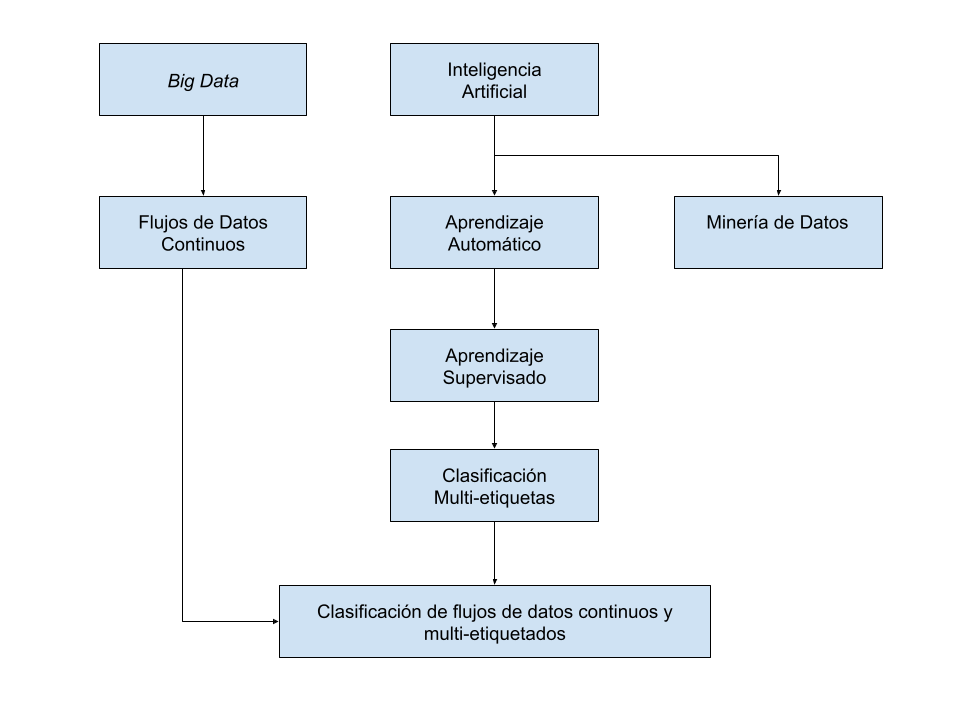
\includegraphics[width=\linewidth]{figures/study_field_taxonomy_v2.png}
  \caption{Taxonomía del campo de estudio}
  \label{fig:campo_estudio}
\end{figure}

